\chapter{Proposed Methodology}
\label{chap3}

In the previous chapter, we have discussed the theories that support this
research related to the University Network using Cisco Packet Tracer. In this chapter we will proposed our methodology for this project.\\\\
Basically we are following the given below question step by step.\\
COMSATS University is a large university which has 4 main buildings situated apart. The university's students and staff are distributed in 4 departments: these includes the Department of Electrical and Computer Engineering, Department of Mathematics, Department of Computer Sciences, \& Admission Office.\\\\
Each member of staff has a PC and students have access to PCs in the labs.\\\\
\noindent {\Large \textbf{Requirements}} \\
\begin{itemize}
\item Create a network topology with the main components to support the following:
    \begin{enumerate}
    \item {\small \textbf{Building A}}: Department of Electrical and Computer Engineering is distributed in the building offices for the faculty, and labs. It is expected that they will share networking equipment ({\small \textbf{Hint: use of VLANs is expected here}})
    \item {\small \textbf{Building B}}: Department of Mathematics including offices, lecture halls/lecture rooms.
%
    \item {\small \textbf{Building C}}: Admission office distributed in different offices.
    \item There is also an email server hosted externally on the cloud.
    \item {\small \textbf{Building D}}: Department of Computer Sciences (CS) this can acts as a smaller campus as well as. It includes different offices and labs.
%
\end{enumerate}
\item You will be expected to configure the core devices and few end devices to provide end-to-end connectivity and access to the internal servers and the external server.
    \begin{enumerate}
    \item Each department/faculty is expected to be on its own separate IP network
    \item The switches should be configured with appropriate VLANs and security settings
    \item RIPv2 will be used to provide routing for the routers in the internal network and static routing for the external server.
    \item The devices in building A will be expected to acquire dynamic IP addresses from a router-based DHCP server
%
\end{enumerate}
\end{itemize}

\section{Block Diagram}
Let us look at the detail block diagram in Figure \ref{blockDiagram}, which illustrates the main components involved
in University Network using Cisco Packet Tracer.\\
In this diagram, we have used:
\begin{enumerate}
    \item 2911 Router, for the main campus network
    \item 3650-24PS Multi Layer Switch, for different departments in the buildings 
    \item 2960-24TT Switches, for each department 
    \item A cloud router,
    \item Servers, email server hosted externally on cloud, and a web server for IT department
    \item Host Devices, a PC and a printer 
    \item Wire, Serial DCE (HWIC-2T) for routers connections, Copper cross over for switches connections, and Copper straight through for the host devices connections.
%
\end{enumerate}
 
\begin{figure}[H]  %h=positioning
\begin{center}
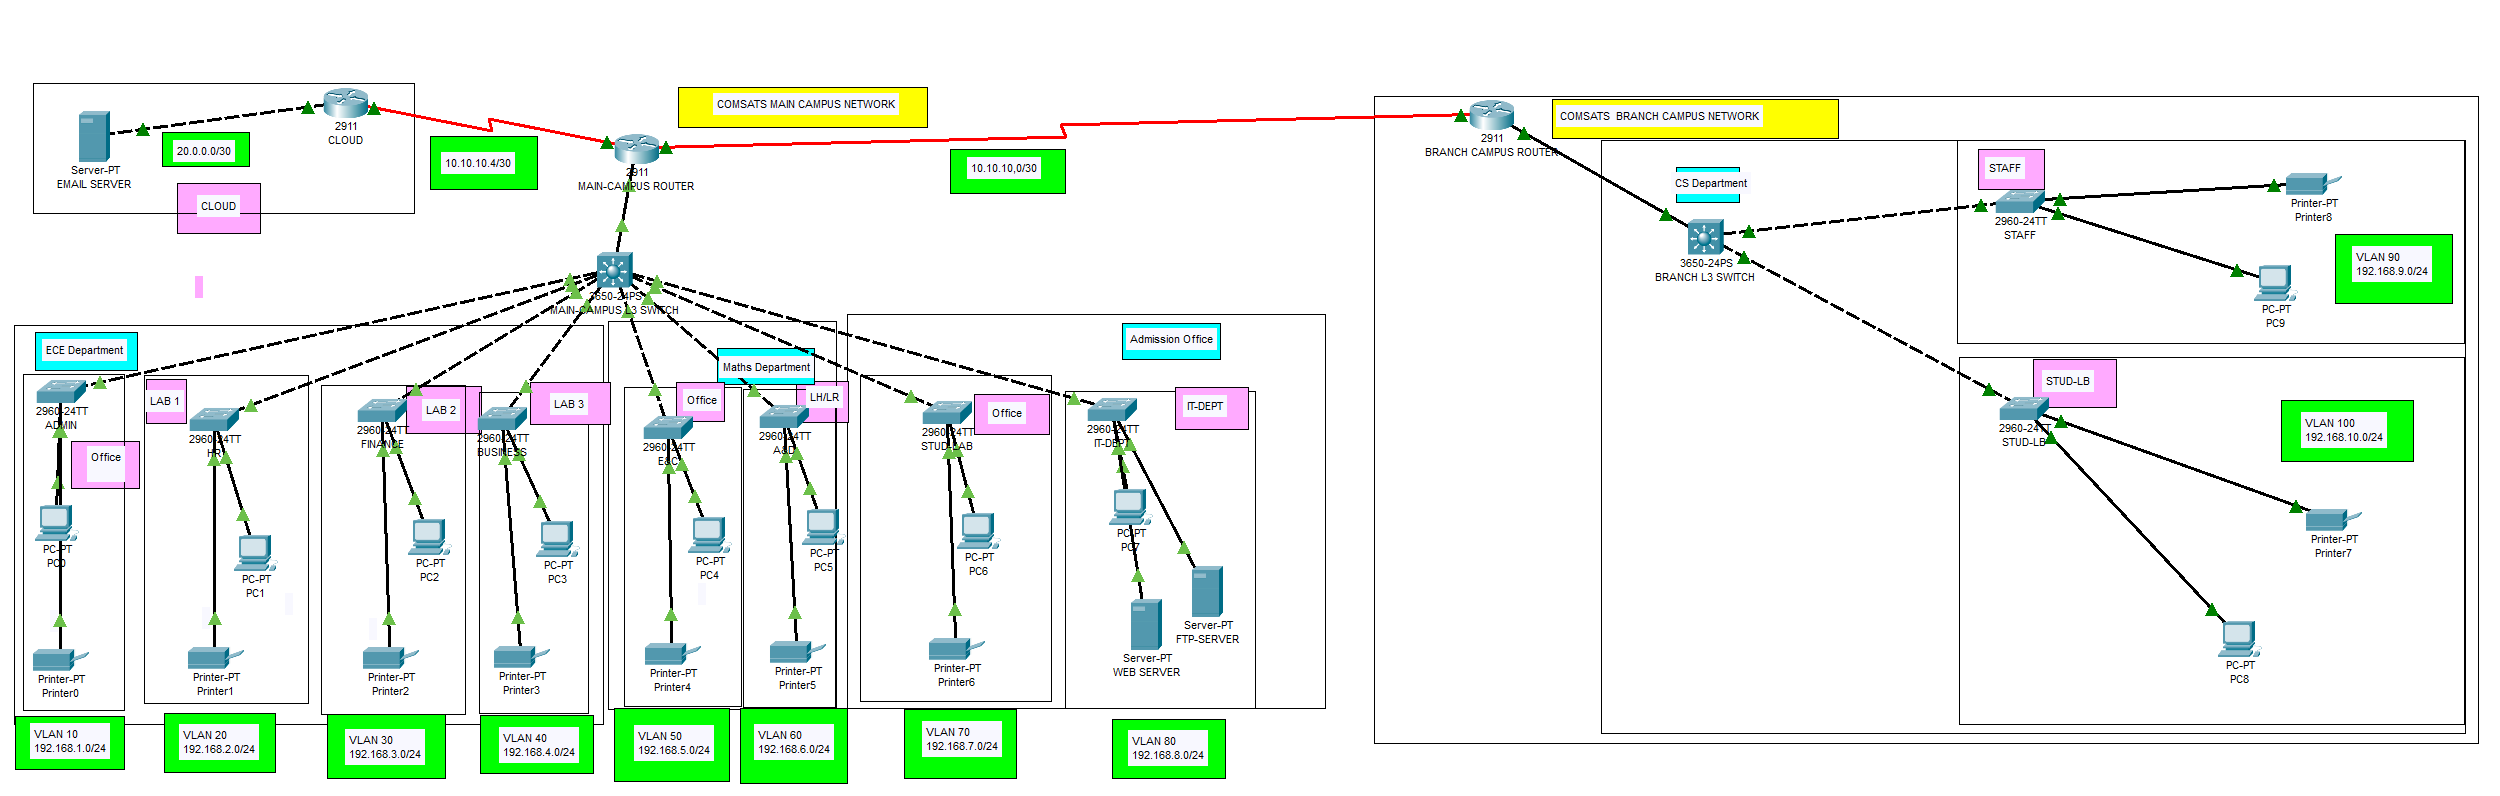
\includegraphics[scale=0.24]{Chapter3/blockDiagram}
\caption{Block Diagram of University Network }
\label{blockDiagram}
\end{center}
\end{figure}

\section{Flow Chart}
Figure \ref{flowChart} shows the flow chart of the University Network. Basically the main objective of the project is the communication between different departments. To do so, we send message from one of the department's pc to any other department's pc or printer.\\\\
We will configure the network first, and than will check out if the IP of the next computer and our computer is working well. It will transfer our message packet to the destination host.
\begin{figure}[H]  %h=positioning
\begin{center}
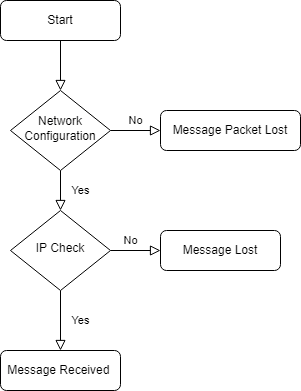
\includegraphics[scale=0.70]{Chapter3/flowChart}
\caption{Flow Chart of University Network }
\label{flowChart}
\end{center}
\end{figure}

\section{System Model}
A large campus with groups of buildings can also use WAN technology to connect the buildings as shown in the Fig. \ref{systemModel}. Although the wiring and protocols of a campus might be based on WAN technology, they do not share the WAN constraint of the high cost of bandwidth. After the wire is installed, bandwidth is inexpensive because the company owns the wires and there is no recurring cost to a service provider. However, upgrading the physical wiring can be expensive.
\begin{figure}[H]  %h=positioning
\begin{center}
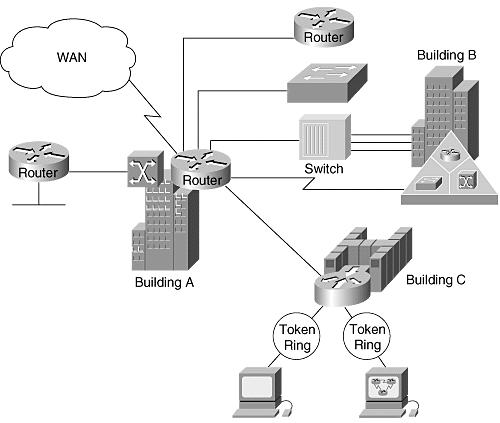
\includegraphics[scale=0.67]{Chapter3/systemModel}
\caption{System Model of University Network}
\label{systemModel}
\end{center}
\end{figure}
\section{Software Selection}
We will simulate our campus network using Cisco Packet Tracer Version: 7.3.0.0838. Cisco Packet Tracer is a powerful network simulator for CCNATM and CCNPTM certification exam training allowing students to create networks with an almost unlimited number of devices and to experience troubleshooting without having to buy real CiscoTM routers or switches.\\

\noindent Cisco Packet Tracer features an array of simulated routing \& switching protocols with STP, HSRP, RIP, OSPF, EIGRP, and BGP to the extent required by the current Cisco CCNA curriculum as well as application layer protocols (HTTP, DNS, �) to simulate network trafic .\\

\noindent It also includes Cisco IOS 15 with licence features, wireless capabilities with WLC and lightweight access point, security devices with ASA 5505 and 5506-X firewalls, and SDN controller.
\begin{figure}[H]  %h=positioning
\begin{center}
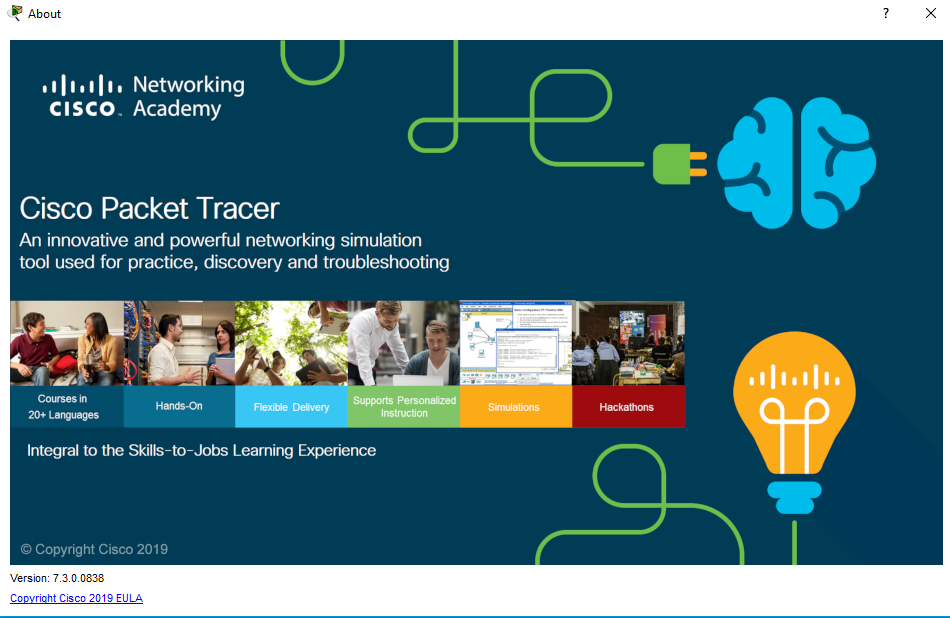
\includegraphics[scale=0.60]{Chapter3/software}
\caption{Cisco Packet Tracer}
\label{software}
\end{center}
\end{figure}

{ \small \bfseries Note: You can simulate this network on any latest version as well as.}


